\documentclass[a4paper, 10pt, conference]{ieeeconf} 
\IEEEoverridecommandlockouts                                                                                    
\overrideIEEEmargins                                      			

\usepackage{graphics} % for pdf, bitmapped graphics files
\usepackage{epsfig} % for postscript graphics files
\usepackage{mathptmx} % assumes new font selection scheme installed
\usepackage{times} % assumes new font selection scheme installed
\usepackage{amsmath} % assumes amsmath package installed
\usepackage{amssymb}  % assumes amsmath package installed
\usepackage{amsfonts}
\usepackage{textcomp}
\usepackage{graphicx}
\usepackage{float}


\title{\LARGE \bf
Review of Standard Rotor Configurations for a Micro Unmanned Aerial System
}

\author{Angus Steele$^{1}$ and Johann Treurnicht$^{2}$% <-this % stops a space
\thanks{*This work was supported by the CSIR}% <-this % stops a space
\thanks{$^{1}$Angus Steele is an employee at the CSIR as well as an MSc Student at The University of Stellenbosch (ASteele@csir.co.za)}%
\thanks{$^{2}$Johann Treurnicht is with the Department of Electronic Engineering, The University of Stellenbosch}%
}

\begin{document}

\maketitle

\begin{abstract}
The use of unmanned aerial systems (UAS) is on the rise with an array of industries finding use for them in a variety of applications. This review hopes to assist potential drone designers in selecting the drone best suited for their application. This paper attempts to first give a better understanding of flight theory and the basics of rotary winged vehicles. Next it builds on that knowledge and applies it to a few important selection parameters, after which it addresses the criteria and links it directly to a few standard configurations of rotorcraft. In the final discussion a few key points are addressed and each standard configuration is discussed in its ideal application.
\end{abstract}
\section{INTRODUCTION}
With the increase in computing power making rotorcraft control possible, drones are becoming an ever more popular platform for a variety of applications and users. From military personnel to photographers, drones are benefiting an array of industries. The hobbyist now can pick and choose from a warehouse full of different rotors, motors and full drone kits. 

There is a lot of documentation available about rotorcraft, especially since they has recently gained a lot of attention from hobbyists. Unfortunately there are not a lot of comparisons between the different types of configurations, nor what parameters should be looked at. This misunderstanding results in many users end up using a drone type that is not the optimal choice for the application. This paper will summarise a few key points of rotor dynamic theory and then use this information to address a few important parameters before finally applying it to different drone configurations. By the end of this paper the reader should be able to identify the appropriate rotor configuration for their application.

\section{FUNDAMENTALS OF FLIGHT THEORY}

\subsection{Basic Rotor Theory}
The rotor is responsible for all the aspects of flight and generates the lift, forward propulsion and the means to control the orientation of the craft \cite{Leishman}. It is for this reason that an in depth understanding of rotor characteristics and performance is needed. Any rotating blade will cause a rotation of the craft in the opposite direction to that motion. This applied moment must be countered by a counter-torque mechanism. This function is performed by the tail rotor in a traditional helicopter.

The capability of any part of a rotor to produce lift is influenced by the local blade position and pressure at that point \cite{Leishman}. As the rotor spins, the blade's angle relative to air stream in shifts as shown Figure \ref{IM_TipSpeed}. This angle is defined as an azimuth angle ($\alpha$) and is measured relative to air flow. The azimuth angle is 0\textdegree\ downstream and sits at 180\textdegree\ when it faces directly upstream. The speed of any part of the rotor varies along the length of the rotor, with the maximum velocity at the rotor tip. Figure \ref{IM_TipSpeed} demonstrates the naming scheme.

As the rotorcraft adds a horizontal component to its hover or vertical flight, the relative speed of the individual rotor segments now adheres to \eqref{EQ_TipSpeed}. The relative velocity at any part of the rotor is affected by the azimuth angle of the blade ($\alpha$), forward translatory speed of the craft ($V_{\infty}$), angular speed of the rotor ($\Omega$) and the considered distance along the rotor blade (r) \cite{Leishman, RotorCraftHand}.

\begin{equation}
\label{EQ_TipSpeed}
V_{r} = \Omega r + V_{\infty}\sin(\alpha)
\end{equation}

What this relationship shows is that during forward flight the tip velocity, relative to the ground, changes even if the rotor rotates at a constant speed. This relationship complicates the rotor dynamics at higher speeds and limits the top speed of the craft. On the retreating edge ($\alpha = 270$\textdegree $\therefore \sin(\alpha) = -1$) if $\Omega r \leq V_{\infty}$ the rotor would effectively be going backwards and the helicopter is at risk of stalling out. This relative speed is known as a stall condition, while the advancing edge is reaching its maximum speed by approaching transonic conditions and severe instability \cite{Leishman, RotorCraftHand}.

\begin{figure}[t]
\centering
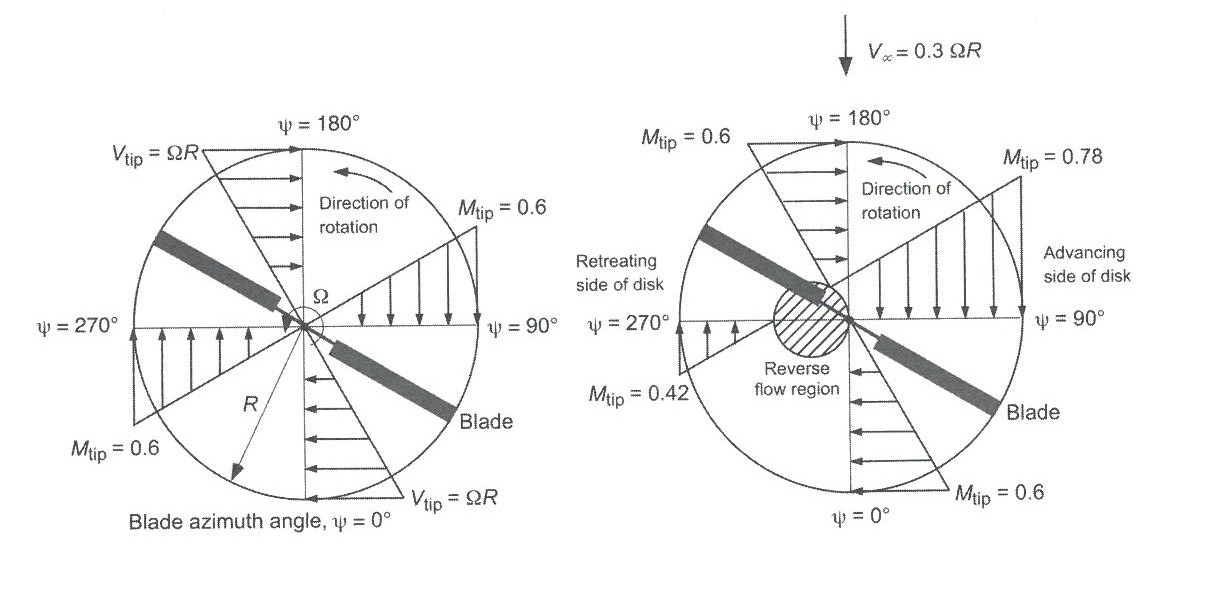
\includegraphics[height = 5cm]{Images/Literature/TipSpeed}
\caption{Velocity components of a rotor (taken from \cite{Leishman})}
\label{IM_TipSpeed}
\end{figure}

\subsection{Momentum Theory and the Basics of Thrust}
As mentioned above, the rotors of a rotorcraft are responsible for generating all the forces that manoeuvre the vehicle. These forces are induced by pushing air through the rotor disk. With a fixed wing aircraft the analysis of the blades is simplified because the only air flow produced is from the translational velocity of the entire craft. Analysis of blade performance in a rotorcraft can be more challenging as the rotation of the blades must be considered alongside the overall speed of the vehicle. As the craft manoeuvres in space, the air flow through the rotor adds significant complexities to the analysis. Since the rotorcraft is expected to perform in a variety of flight styles it is important to understand these models as well as their flaws. 

\begin{figure}[t]
\centering
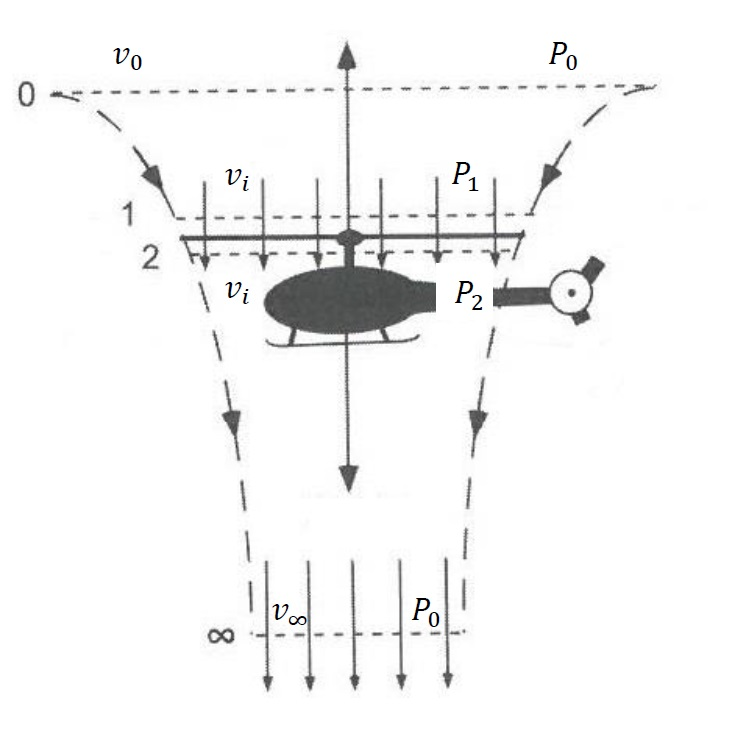
\includegraphics[height = 5cm, angle=360]{Images/Literature/MomentumTheoryHover}			%Must show both air flow as well as far stream and such
\caption{Momentum Theory in Hover (adapted from \cite{Leishman})}
\label{IM_MomentumTheoryHover}
\end{figure}

Thrust is the name given to the collective vector with lift being the component that opposes the weight, for simplification the helicopter is considered to be in a state of hover (weight = lift = thrust). The rotor 'smooths' out the air as it forces it through the disk area. This more uniform air creates an edge known as the slipstream or wake boundary, with the surrounding air remaining dormant \cite{Leishman}. Inside the wake boundary, the average velocity of the air is tangible, where outside the slipstream edge, the average air velocity is negligible. The force required to push that mass of air through the disk space is, by Newton's third law, returned by the air to the rotor, thus giving the rotor blades a thrust component. 

Rankine-Froude's Momentum Theory looks at this induced velocity as well as the displacement of air through the propeller, and attempts to quantify the induced thrust. The variable naming convention for the equations is shown in Figure \ref{IM_MomentumTheoryHover} above and is adopted from Leishman et al \cite{Leishman} in their naming of the components. Subscripts 0, 1, 2 and $\infty$ refer to the locations of quiescent flow, inflow directly before the rotor, airflow immediately after the disk and the slipstream\footnote{Generally far wake is considered as 1 full rotor diameter distance away \cite{Leishman}.} or far wake condition respectively. The velocities are shown as the induced velocity in and out the rotor ($v_{i}$), the far wake velocity ($v_{\infty}$) and finally $v_{0}$ represents the zone with zero flow rate. There is no velocity discontinuity across the rotor, the energy being fed into the system by the rotor is represented by a pressure change between $P_1$ and $P_2$.


As described above, it is by forcing the air through the disk that lift is generated. The mass flow rate of this air can then be described by (\ref{EQ_MassFlow}), where $\rho$ is the density of air and A is the area of one full blade rotation. The rate at which this mass of air is displaced becomes a crucial variable in rotor dynamics and is directly proportional to thrust (T). This relationship can be quantified as shown in (\ref{EQ_ThrustBasic}). Thrust can also be calculated by finding the difference in pressures over the rotor disk as in (\ref{EQ_ThrustPressure})

\begin{eqnarray}
\dot{m} &=& \rho A v_{i}\label{EQ_MassFlow}\\
T &=& \dot{m}a\label{EQ_ThrustBasic}\\
T &=& A(P_2 - P_1)\label{EQ_ThrustPressure}
\end{eqnarray}

Since $v_0$ is zero during hover and acceleration is the difference in $v_\infty$ and $v_0$, (\ref{EQ_ThrustMass}) can be obtained.

\begin{equation}
\label{EQ_ThrustMass}
T = \rho A v_{i} v_\infty
\end{equation}

Thrust can now be quantified once the slipstream and induced velocities are known. Then by applying Bernoulli's equation of conservation to both sides of the rotor disk, the change in pressure across the disk can be quantified as shown in (\ref{EQ_Bernoulli2}).
That change in pressure fits into one of the initial definitions of thrust (\ref{EQ_ThrustPressure}). Equating both of those definitions yields an important relationship between the three velocities, as shown in (\ref{EQ_RotorVelocity}). The relationship simply states that the induced velocity at the rotor is the average of the quiescent flow above and the far wake velocities. This definition proves useful at a later stage in the rotor theory definitions. 

\begin{eqnarray}
P_2 - P_1 &=& \frac{1}{2} \rho (v_\infty^2 - v_0^2)\label{EQ_Bernoulli2}\\
v_i &=& \frac{1}{2} (v_\infty + v_0)\label{EQ_RotorVelocity}
\end{eqnarray}


\subsection{Disk and Power Loading}
Disk loading (DL) is a term seen often in the world of rotorcraft, and describes a simple but important ratio between thrust and the area a rotating disk covers. It is represented in its simplest form in the beginning of \eqref{EQ_DL} and is measured in $\frac{N}{m^{2}}$. Since the pressure drop across each rotor is considered uniform, the disk loading for each rotor will equate to the pressure drop across that disk. Equation (\ref{EQ_Bernoulli2}) first shows the difference in pressure and by taking $v_0$ as zero (state of hover), the second half of equation (\ref{EQ_DL}) can be formed. 
\begin{equation}
\label{EQ_DL}
DL = \frac{T}{A} = \frac{1}{2} \rho v_\infty^2
\end{equation}

\begin{figure}[b]
\centering
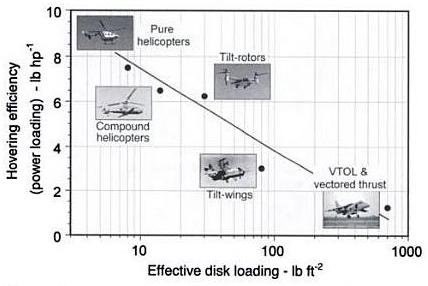
\includegraphics[height = 6cm]{Images/Literature/DL}     
\caption{Image representing, various Disk Loading values for varying rotorcraft (Taken from \cite{Leishman})}
\label{IM_DL}
\end{figure}

For multi-rotor craft, the disk loading is assumed uniform across all rotors \cite{Leishman}. The overall disk loading of a single rotor craft such as a traditional helicopter will be lower than that of a multi-rotor craft of a similar size \cite{RotorCraftHand}. Figure \ref{IM_DL} shows some examples of disk loading values for a variety of rotor configurations, as shown, disk loading is also a measure of hover efficiency.
A higher disk loading value results in larger values for induced velocities as well as the required power to hover. This relationship means that the larger the blades, the better the efficiency. More force will be generated by pushing large quantities of air slowly than forcing small amounts of air through at high speeds \cite{TheoryofFlight}. With bigger blades comes larger rotational inertia and geometry. The craft is also less immune to gusts and interferences. A larger blade creates faster tip velocities which will limit the speed of the craft severely \cite{Leishman}.

Power is given by the product of thrust and the induced velocity at the blade. It can be written as shown in (\ref{EQ_Power}). What this ratio shows is that the ideal power is in cubic proportion to the induced velocity at the rotor. Therefore to reduce required power the rotors induced velocity must be small, which can be accomplished by an increase in disk area \cite{Leishman}.

\begin{equation}
\label{EQ_Power}
P = 2 \rho A v_{i}^3
\end{equation}

Another important ratio is between thrust and power. It is called power loading (PL) and is shown in (\ref{EQ_PL}). Power loading can be seen as a measure of craft efficiency and is measured in $\frac{N}{kW}$. 

\begin{equation}
\label{EQ_PL}
PL = \frac{T}{P}
\end{equation}

From  \eqref{EQ_DL} and \eqref{EQ_PL} it can be shown that power loading is inversely proportional to disk loading. Therefore a craft with lower disk loading will be a more efficient platform.

\subsection{Electrical Power to Thrust}
Equation (\ref{EQ_Power}) gives a quantitative approach to solving for aerodynamic power ($P_i$). If electrical power is taken as $P_e = VI$, where V is the applied voltage and I is the sourced current, with an efficiency of $\eta$ then $P_i = \eta VI$. Noting that $P_i = T v_i$ and using (\ref{EQ_Power}), a relationship between thrust and $P_e$ can be formed and is represented in (\ref{EQ_ElectricalPowerThrust}).

\begin{equation}
\label{EQ_ElectricalPowerThrust}
T = (2\rho A)^{\frac{1}{3}} (\eta P_e)^{\frac{2}{3}}
\end{equation}

Equation (\ref{EQ_ElectricalPowerThrust}) brings to light a very important relationship which states that thrust grows at a slower rate than the electrical input power to the system.

\begin{equation*}
T \propto P_e^{\frac{2}{3}}
\end{equation*}

\section{SELECTION PARAMETERS}
Some of the fundamental theories described above relate to the basics behind various rotor configurations and even varying flight techniques. Each different arrangement of blades introduces certain advantages and disadvantages to the system. Not every configuration will be applicable for all operations and it is important to determine what criteria are critical for the intended application.  An analysis of varying rotor configurations is done below and follows a similar trend to that seen in \cite{RotorConfig}, \cite{Bohorquez} and \cite{NewMAV}. The main weighted criteria for the discussion were listed in no particular order as:

\begin{enumerate}
	\item Flight time, payload capability and efficiency
	\item Geometry, size and mechanical complexity
	\item Drone manoeuvrability and control algorithms
	\item Stability and disturbance rejection
\end{enumerate}

\subsection{Efficiency, Payload Capability and Flight Time} 
Flight time is a by-product of efficiency and payload, as a more efficient craft will drain the power source slower, thus producing a longer flight. A heavier craft, with a larger payload, will have a shorter flight duration. Most miniature drones today have a flight time between 6 - 12 minutes before they need recharging. This length is not suitable for a variety of applications where longer mission durations are pertinent. A larger power source could always be added, but will increase the weight, limiting the payload capability and once again flight time. The relation between hover efficiency and disk loading was mentioned above, but what was not discussed is how a potential payload affects these decisions. With no payload a single rotor will have a lower disk loading and will not be able to carry as heavy loads as a multi-rotor craft that has a higher disk loading \cite{Leishman, Camrad, RotorCraftHand}.

\subsection{Geometry, Size and Mechanical Complexity}
In any aerial vehicle mass is always an important design criterion. Every aspect of the platform must be designed to be the lightest it possibly can. Having a light weight craft is one part of the design criterion, another would be ensuring that the weight is geometrically spread out correctly, as well as functionally distributed appropriately. The table below was adapted from \cite{NewMAV} and demonstrates the latter point. Depending on the different criteria for the craft, different functional blocks will be allocated a certain percentage of weight. For example, if the user would like a longer flight time, a higher percentage would be given to the power source and possibly less to the external payload. Generating a good mass model before designing helps better understand the requirements for the craft and could be a deciding factor in the construction.

\begin{table}[H]
\centering
\begin{tabular}{l | c | c | c | c}

Component 					& 0.3kg & 1.8kg & 3.7kg\\
\hline\hline
Rotor System 				& 11.0 & 11.2 & 13.9\\
Tailboom Assembly 		& 8.0 & 9.1 & 7.8\\
Main Rotor Motor 			& 15.4 & 10.5 & 8.1\\
Fuselage/Structure 			& 7.0 &  15.1 & 12.0\\
Main Transmission 			& 2.0 &  3.4 & 3.4\\
Landing Gear 				& 2.3 &  3.4 & 2.9\\
Control System 				& 5.7 & 18.3 & 9.3\\
Avionics 						& 29.4 &  2.4 & 1.6\\
Power Source 				& 19.2 & 26.6 & 41.0\\

\end{tabular}
\caption{UAS Weight Data (Adapted from \cite{NewMAV})}
\end{table}

It was also mentioned that the weight needs to be geometrically positioned correctly, the point of this would be to create as much symmetry in the craft as possible. If this is done correctly the principal axes of inertia will align very closely with the body of the craft. The inertia tensor is a matrix that is a representation of a rigid body's resistance to movements in three dimensional (3D) space.  For the general case the inertia tensor takes the form as shown in \eqref{EQ_InertiaTensor}. The inertia tensor is very dependant on a craft's symmetry, and is symmetric itself. In other words, $I_{xy} = I_{yx}$, $I_{xz} = I_{zx}$ and $I_{zy} = I_{yz}$ and therefore if a craft is symmetric about the y axis (x = 0), then $I_{xy} = I_{yx} = 0 = I_{xz} = I_{zx}$ \cite{Luukkonen, MiniFlying}.

\begin{equation}
\label{EQ_InertiaTensor}
\textbf{I} = 
\begin{bmatrix}
I_{xx}	& -I_{xy} & -I_{xz}\\
-I_{yx}	& I_{yy}	& -I_{yz}\\
-I_{zx}	& -I_{zy}	& I_{zz}\\
\end{bmatrix}
\end{equation}

Symmetry in a craft can also help reduce the effects of disturbances such as mechanical drag and even wind. More on disturbance rejection is mentioned below.

\subsection{Drone Manoeuvrability and Control Algorithms}
In 3D space there are effectively six possible degrees of freedom (DOF) three of which are translational ($\boldsymbol{\xi}$) and three of them rotational ($\boldsymbol{\eta}$). The naming scheme used in this paper follows the same form used by Castillo et al in \cite{MiniFlying, RealTime}. In mathematics there are discussions regarding rotations around the x, y and z axes, though in flight theory they are labelled as roll, pitch and yaw. The three axes change as the aircraft's orientation changes since they are labelled relative to the aircraft's position. Pitch relates to how much the vehicle is tipping forward or backward, roll is an influence in the left and right rotation, while yaw is rotation around the z axis. Instead of  x, y and z, these axes can be considered as forward, sideways and normal \cite{Leishman}. Refer to Figure \ref{IM_PRY} for a visual description of the axes.

\begin{figure}[b]
	\centering
	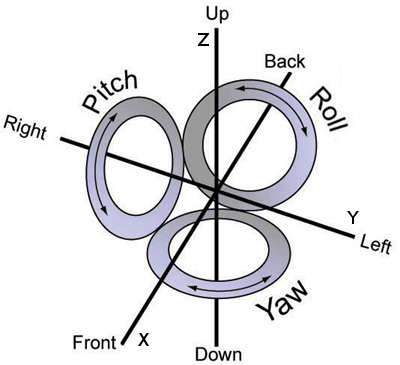
\includegraphics[height = 5cm]{Images/Literature/RollPitchYaw}     
	\caption{Control surfaces required for 3 dimensional flight (Taken from \cite{Heli})}
	\label{IM_PRY}
\end{figure}

\begin{eqnarray}
\boldsymbol{\xi}= 
\begin{bmatrix}
x\\
y\\
z
\end{bmatrix}&
\boldsymbol{\eta} = 
\begin{bmatrix}
\phi\\
\theta\\
\psi
\end{bmatrix}& 
\textbf{\textit{q}} = 
\begin{bmatrix}
\boldsymbol{\xi}\\
\boldsymbol{\eta}
\end{bmatrix}
\label{EQ_InertiaFrame}
\end{eqnarray}

Drone manoeuvrability and control algorithms have been grouped together because they both relate directly to the dynamic model of the craft, as well as the amount of control authority available to the pilot. The same way that the wheels in a car decide which direction the car drives, the rotors provide all the control authority to a standard rotorcraft. Having only a single, fixed pitched rotor allows only for control in the amount of upwards and downwards acceleration the craft has. There are many different methods to obtain full six degrees of flight freedom. 

Typically a rotorcraft will be designed with either fixed pitched, or variable pitched rotors. A fixed pitched rotor is a rotor that has an optimally selected, unchangeable pitch and therefore a fixed angle of attack. This means that since the angle of attack is fixed for the blade, an increase in RPM will be required for a change in lift. With a variable pitched blade, the pilot can change the angle of attack to increase the forces. As the angle of attack increases, the blade will produce more lift without changing the speed of the motor. However, as the pitch increases, so does the drag of the blade. This drag then requires more motor power to keep the blade moving through the air \cite{MiniFlying, Leishman}. 

The power requirements for either system are fairly similar; though the advantages of a varying pitch is that a single rotor has the potential for more dynamic force applications. The downfall however is the high level of complexity in the mechanical design. Both of these facts become pertinent in the final platform design. The end goal is to have a craft that can fly stably and accurately in three dimensions. To do this the craft will need more control surfaces to apply forces in those planes. There are many different methods to obtain the full six degrees of flight freedom. Some designers have added multiple rotors, ensuring there is always a counter rotating pair which eliminates the anti-torque generated by each motor. Ultimately giving the engineer more control authority will simplify the control algorithms and increase drone manoeuvrability. Having only a single, fixed pitched rotor will allow only for control in the amount the craft flies up or down, as well some instability in the system. 

Most configurations will give the user sufficient control authority, the trade off becomes between number of rotors and mechanical complexity.


\subsection{Stability and Disturbance Rejection}
Stability and disturbance rejection are generally considered control problems and a good control system can stabilise the craft amongst disturbances. These parameters have been isolated in this case to focus on what can be done before there is an attempt to apply control theory. 
Stability is a broad term and what is meant by it in this case is the ability to completely control movements in all six DOF. Any rotating member will produce a counter rotating torque to the static body, which means that any system with only one fixed pitched rotor will have inherent instability in the yaw axis and only vertical control \cite{MiniFlying}. 
It was mentioned earlier that symmetry in the craft can help eliminate the effects of some disturbances. Multiple blades helps reduce the effects of disturbances just as well. This way if one rotor falters or is affected substantially by a disturbance the other rotors can still rectify the error. Some multi-rotor designs can still fly with substantial control even after losing power to one or more of the rotors \cite{RotorLoss}. 


\section{DISCUSSION}
This discussion looks at the different rotor configurations and attempts to address each parameter mentioned above. It begins with the traditional helicopter which is always seen as a main rotor with a smaller rotor at the tail, even when there are many different types of anti torque tail set-ups. The ducted fan approach reduces the risk of damaging the tail rotor while silencing the system. The NOTAR design \cite{US4200252} manipulates the airflow generated by the main rotor and directs it to counter act the induced torque. A tip-jet design eliminates the torque applied to the airframe and therefore no tail rotor is required \cite{RotorConfig}. There have been many attempts at improving the standard helicopter design. These improvements have taken the form of adding rotors, designing hybrid aircraft and complex mechanical designs to harvest advantages of both the fixed wing and vertical take off and landing (VTOL) craft. Some have even tried to combine multiple features as Flanigan \cite{US7147182} did in his design of a tip-jet, compound, tilt rotor aircraft. 

In an attempt at simplification, not all configurations were investigated. The following standard groups of designs were covered:

\begin{enumerate}
\item Traditional helicopter
\item Coaxial rotors
\item Tandem rotors
\item Multirotor designs
\item Tilt rotors 
\end{enumerate}

\subsection{Traditional Helicopter}
When most people think of a rotorcraft they will think of a conventional helicopter, which is still the most widely used configuration for large rotorcraft \cite{RotorConfig}. It consists of a single main rotor, coupled with a smaller rotor located in the tail to counter act the developed counter torque.

The main rotor of a standard helicopter has very low disk loading which gives it excellent hover efficiency. To achieve yaw stability this configuration makes use of a small tail rotor to counter act the induced moments of the main rotor. The extended tail rotor requires energy which it will draw from the motor while also adding a significant amount of length to the craft. Since the single rotor only gives the pilot thrust control and the tail rotor gives measurable yaw control, there is need for more control surfaces to do more manoeuvring. Most helicopters use a variable pitched rotor system. Cyclic control of this pitch allows the pilot to adjust the angle of attack of the rotor blades while they rotate. This set up is mechanically very complex but luckily has become a standard production set up, with many companies providing solutions to this problem. 

Once the mechanics are set up the control algorithms are still slightly limited and intensive. However with only a single main rotor the traditional helicopter is extremely susceptible to disturbances and has a limited payload capability with the low disk loading factor. The need for the tail-boom assembly also adds significant length to the craft.

\subsection{Coaxial Rotors}
A coaxial configuration consists of two counter rotating blades located about the same centre of rotation that both use the same drive system. This counter rotating pair eliminates the need for a tail rotor as the torque applied by both rotors cancel. Functionally the coaxial is very similar to the traditional helicopter \cite{NasaCoaxial}. With no modifications and only using fixed pitched rotors, this platform will only give yaw and over all thrust control. Bohorquez et al \cite{Bohorquez} attempted a number of lateral control methods, eventually settling on aerodynamic flaps to control the flow of the downwash. That, and other methods, are shown in Figure \ref{IM_Coaxial_Variations}. Briod et all also used the same set up in his team's design of the Gimball \cite{Briod2012}.
 
\begin{figure}[b]
	\centering
	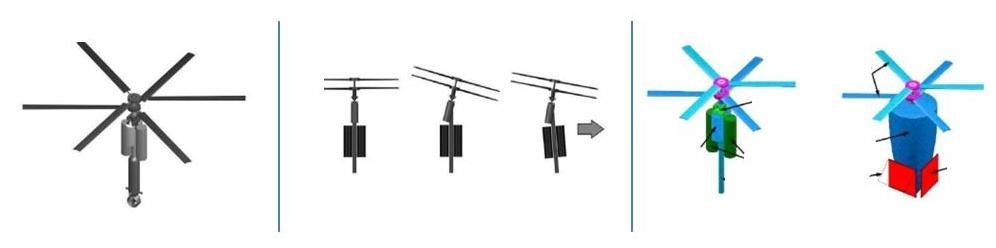
\includegraphics[height = 2cm]{Images/Literature/Coaxial_Configs}     
	\caption{Different methods of lateral control in a Coaxial UAS (Adapted from \cite{Bohorquez})}
	\label{IM_Coaxial_Variations}
\end{figure}

The control flaps are the most common form of lateral control for a small coaxial UAS. They introduce little mechanical complexity and do not require excessive power to use. The flaps do however decrease efficiency of the system, but if designed correctly should only influence the system while being used. For hover and vertical flight the impact will be negligible. As a control surface the flap is quite rudimentary and will require more advanced control methods as well as in depth testing to obtain smooth flight transitions. Due to its compactness the design can have considerable manoeuvrability if the control algorithms are designed effectively. Each flap will require an actuator, which will increase total weight, power consumption and required mechanics.

Since the bottom rotor is working in the top blades slipstream, it will have a higher $v_0$ and therefore a larger $v_i$, which according to equation \ref{EQ_ThrustBasic} will induce a larger thrust. This coupling relates to high values of efficiency and lower values of disk loading, decreasing the payload capability. Coleman in \cite{NasaCoaxial} did an extensive survey of coaxial rotors and also found that they produce more drag than the conventional rotor set up, which becomes pertinent at higher speeds.

Localising the blades around a single point also helps with the geometry of the craft as it is a more compact design. Briod et al \cite{Briod2012, Klaptocz2010, Collision} used this to their advantage when they were designing a collision resistant robot. The compact design allowed them to surround the entire craft in a rolling protective cage. The set-up of the coaxial main rotors do make the craft vulnerable to disturbances \cite{NasaCoaxial}.

\subsection{Tandem Rotors}
A tandem rotorcraft is sometimes referred to as a dual rotor, as it consists of two blades to generate lift and decrease disk loading while increasing the payload lift capacity. In a tandem configuration the blades sit in the front and the rear of the craft, sometimes slightly overlapping. Tandems are often used in applications that require heavier loads than the traditional helicopter can effectively offer. In a tandem configuration the blades spin in opposite directions to counteract the other one's rotational torque. To obtain control in all wanted degrees of freedom the tandem requires the use of variable pitch rotors, similar to the system used in a traditional helicopter. In the case where the rotors overlap, a tandem helicopter has the problem of its rear rotor being influenced by the wake of the front rotor \cite{Camrad}. Running both rotors at a constant speed limits the chance of fatal rotor collision.

As described in (\ref{EQ_ElectricalPowerThrust}) the thrust of the system increases slower than the electrical power input into the system. In a standard configuration, doubling the electrical power would only increase the thrust by a factor of $\approx 1.587$. Whereas doubling the amount of rotors being driven will double both the thrust and the electrical power. This relationship gives the tandem arrangement the capability of lifting heavier loads with relatively low power consumption, as well as demonstrating low power consumption for hover and slow translatory flight. Having twin blades does increase the size of the craft, but the elimination of the tail rotor sees the size being similar to that of a classic helicopter. Using two blades also decreases the effects of interferences such as gusts on the craft. 

Coupling of the two gear boxes helps prevent inter-rotor collisions but that does not negate the need for two rotors requiring cyclic control, creating a system that requires complex control.

\subsection{Multirotor Designs}
Drones have joined other remote controlled vehicles in the world of hobbyists. Of all the different designs, the multirotor is the most popular. Through discussions with drone designers and aerial photographers, the four rotor design is generally chosen due to its incredible stability, manoeuvrability and disturbance rejection.

A quadrotor consists of two pairs of counter rotating propellers. Each shaft will be driven by its own motor and unlike the flaps in a coaxial system, every motor in a quadcopter attributes to the lift vector. Having the freedom to control each blade independently gives the pilot advanced manoeuvrability, with minimal mechanical complexities. This configuration also reduces the complexity of the control algorithms as four degrees of freedom can be obtained by simply adjusting the speed of the motors, with two secondary DOF. The multirotor can even rotate on the spot without any change in altitude \cite{ThrustCritical}. 

The quad does however have very high disk loading due its utilisation of rotor space, Figure \ref{IM_CounterBlades} demonstrates the concept. Imagine a traditional helicopter with radius $R = 100$ which creates an area $A = \pi \times 100^2 $, to fit 4 rotors in the same area, without over lap would require a rotor radius of $r < \frac{R}{2} \approx 40$ relating to a total area of $4  \pi \times 40^2$, reducing the total disk area by about 1.5. This reduced disk area with the increase in weight relates to a higher disk loading and a less efficient hover; thus a more power hungry system. Similar to the tandem the increase in number of rotors increases the payload capacity of the multirotor and allows it to lift heavy loads. There are even products that have eight rotors to seriously increase the payload capability \cite{Octocopter}.

Besides the poor hover efficiency, the biggest downside of the multirotor designs is their size and weight. Each blade requires a drive system and space to rotate without interference.

\begin{figure}[t]
\centering
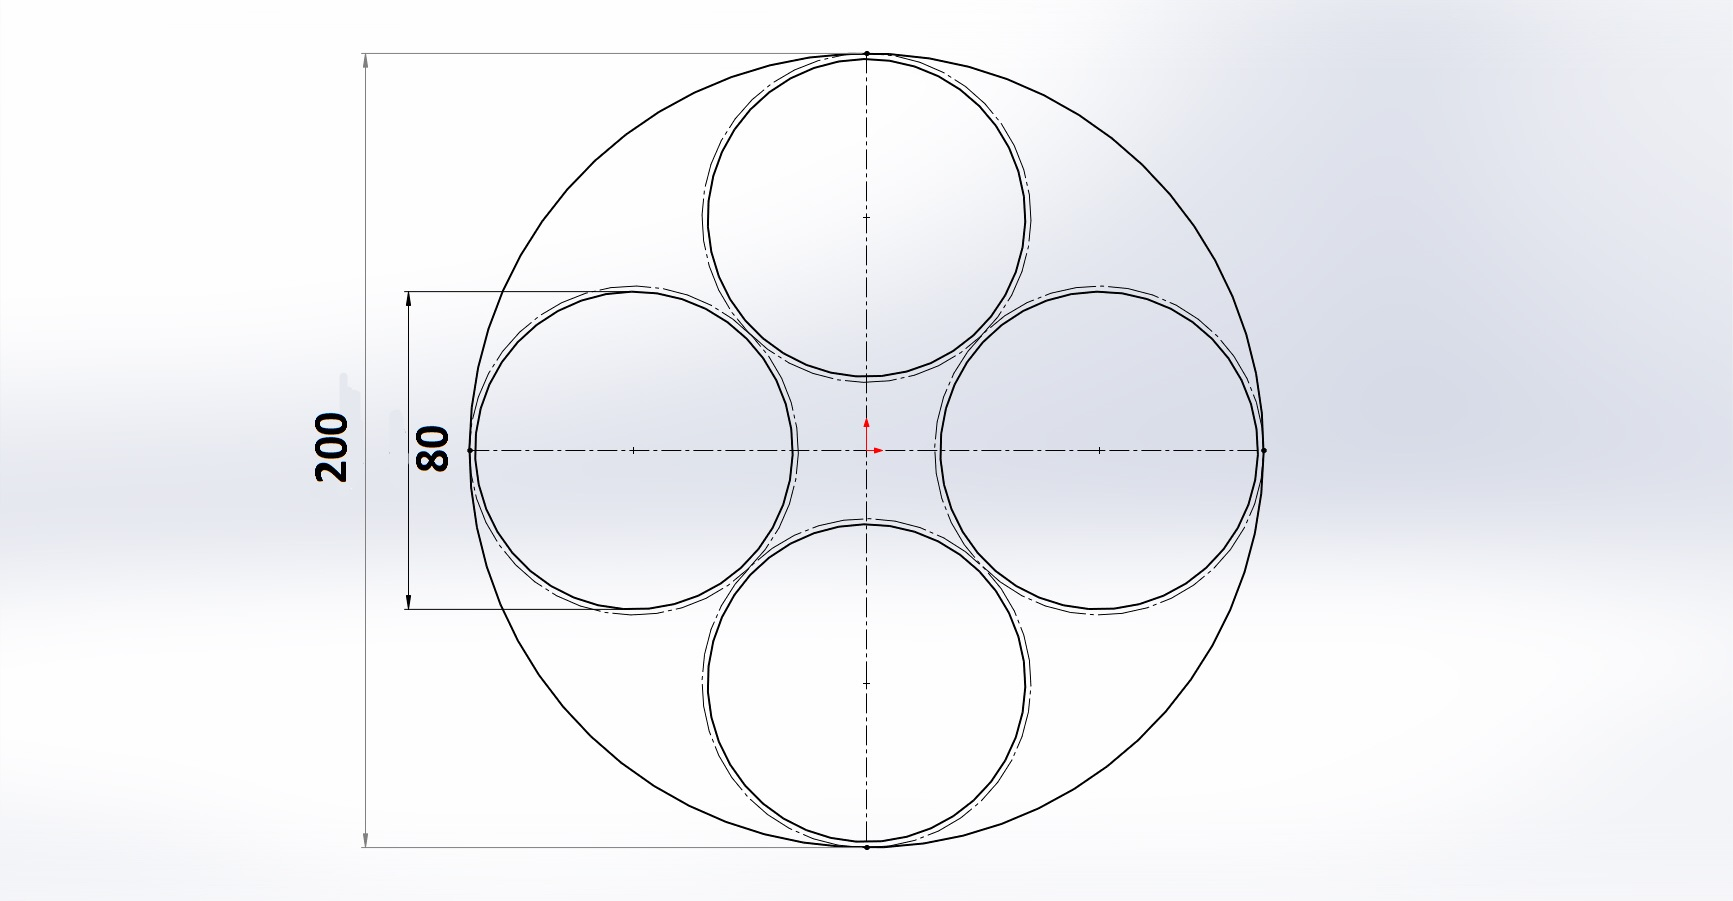
\includegraphics[height =4cm]{Images/Literature/Quad}
\caption{Quadrotor vs Helicopter Rotor Spacing}
\label{IM_CounterBlades}
\end{figure}

\subsection{Tilt Rotors}

A tilt rotor is a very sophisticated system that attempts to harness the benefits of both the fixed and rotor wing aircraft. With the addition of a pivoting axis for each blade the craft has the forward flying speeds of a fixed wing craft while still being able to take off and land vertically like a rotorcraft. The tilt rotor's major downfall is related to the required highly complex and intricate mechanical design \cite{RotorConfig}.
 
VTOL applications require a larger blade to decrease the disk loading, while in forward flight a smaller diameter blade is desired to increase the efficiency of propulsion. Hager \cite{US6030177} developed a telescopic system that transforms the blades to get the optimal benefits out of each configuration. These and other improvements have established the tilt rotor as a competitive design in the field of aeronautic transportation \cite{RotorConfig}. The main advantage of the VTOL system compared to other rotorcraft is the flight efficiency in longer flights. 

%\begin{table}[!]
%\centering
%\label{TAB_PlatformDesign}
%\begin{tabular}{l | c | c | c | c | c | c |}
%Factor 								& Name & Heli & Co & Dual & Multi & Tilt\\
%\hline\hline
%Hover Efficiency 	   				 & 2 & 8 & 8 & 6 & 3 & 2\\
%\hline
%Payload Capabilities	 	  	  & 4 & 5 & 4 & 7 & 9 & 2\\
%\hline
%Physical Size 		       			& 1 & 5 & 9 & 5 & 3 & 5\\
%\hline
%Manoeuvrability 	  	   		   	& 3 & 5 & 4 & 6 & 9 & 2\\
%\hline
%Control Algorithms  			  & 3 & 4 & 4 & 6 & 8 & 4\\
%\hline
%System Simplicity 				 & 3 & 3 & 5 & 7 & 6 & 2\\
%\hline
%Flight Distance						& 3 & 6 & 4 & 5 & 4 & 10\\
%\hline
%Disturbance Rejection 			& 5 & 4 & 3 & 5 & 7 & 4\\
%\hline
%Stability 								& 5 & 5 & 5 & 6 & 8 & 5\\
%\hline
%Top Lateral Speed 				& 1 & 5 & 3 & 6 & 7 & 10\\
%\hline\hline
%Total Score 				& 300 & 145 & 135 & 178 & 208 & 126\\
%\end{tabular}
%\caption{Rotor Configuration Scoring Matrix for an Aerial Photography Platform}
%\end{table}

%Table 2 below is an example of a weighting matrix that tries to summarise the points discussed above, the example is for a drone used for aerial photography. The weighting values will be different for each application.

   
\section{CONCLUSION}
From the above discussion it can be seen that there is no single configuration that is best suited for all applications. Instead each set up has its own pros and cons which can be utilised in different situations. To conclude this review, each standard configuration will be discussed in its ideal application.

Starting with the most application specific, the tilt rotor will only be the most advantageous in a situation that requires flight duration over long distances. With the added need of VTOL, the tilt rotor will trump the conventional fixed wing design. As expected the tilt rotor is also the best choice when it comes to top lateral speed.

The traditional helicopter and the coaxial fulfil a very similar role. They can be sensitive to disturbances and can't handle the payload their multirotor relatives can. However, their hover efficiency is very high which gives them a significant flight time and that's where the traditional set-up earns its place. When an application's main criteria is extended flight time, these should definitely be considered. The choice between coaxial and traditional comes mainly down to size and flight speed. The coaxial will be able to fit in more refined spaced without the additional tail boom assembly, while the traditional will be able to reach higher speeds and fly laterally more efficiently.

The multirotor is the easiest to use, can take the biggest payload and is the most stable, but it will have a shorter flight duration as it is a power hungry system. For the case of the aerial photography it is no surprise that the multirotor was chosen as the best choice as flight duration is not as important to a photographer as stability would be. The multirotor is also the easiest to control which makes it the ideal hobbyist platform.

The tandem has often been cast aside as a suitable configuration \cite{MiniFlying}, mainly because it sits between the traditional and the multirotor on effectively every parameter. So generally one or the other is chosen and the dual rotor set up is neglected. The tandem is suitable for an application that needs a jack of all trades solution. It is a slightly simpler system and will provide a larger payload than the traditional helicopter, while it still has better hover efficiency and overall size compared to the multi-rotor.


\addtolength{\textheight}{-12cm} 

\section*{ACKNOWLEDGMENT}
The authors of this paper would like to extend a thank you to the Council of Scientific and Industrial Research (CSIR) for allowing the space and resources to conduct this study, as well as The University of Stellenbosch for all the advice and direction.

%BIBLIOGRAPHY COMMANDS
\bibliographystyle{plain}
\bibliography{Masters}
\end{document}
